\documentclass{article}

\usepackage{lipsum}
\usepackage[margin=1.5in]{geometry}
\usepackage{titlesec}
\usepackage{graphicx}
\usepackage{amsmath}

\usepackage{mathtools, amssymb, nccmath}
\usepackage{bigstrut, changepage, lipsum}

\newcommand{\code}{\texttt}
\newcommand{\norm}[1]{\left\lVert#1\right\rVert}

\usepackage{siunitx} % Required for alignment


% Specify images directory
\graphicspath{ {./report-images/} }

% Header and Footer stuff
\usepackage{fancyhdr}
\pagestyle{fancy}
\fancyhead{}
\fancyfoot{}
\fancyfoot[R]{ \thepage\ }
\renewcommand{\headrulewidth}{0pt}
\renewcommand{\footrulewidth}{0pt}
\newcommand{\sectionbreak}{\clearpage}
\setlength{\parindent}{0pt}

%

\begin{document}

%----------------------------------------------------------------------------------------
%	TITLE PAGE
%----------------------------------------------------------------------------------------

\begin{titlepage} % Suppresses displaying the page number on the title page and the subsequent page counts as page 1
	\newcommand{\HRule}{\rule{\linewidth}{0.5mm}}% Defines a new command for horizontal lines, change thickness here
	
	\center % Centre everything on the page
	
	%------------------------------------------------
	%	Headings
	%------------------------------------------------
	
	\textsc{\Large Random Number Generation and Simulation}\\[0.5cm] % Major heading such as course name
	
	\textsc{\large Exercise 8}\\[0.5cm] % Minor heading such as course title
	
	%------------------------------------------------
	%	Title
	%------------------------------------------------
	
	\HRule\\[0.6cm]
	
	{\huge\bfseries Area estimation using Monte Carlo method}\\[0.25cm] % Title of your document
	
	\HRule\\[1.5cm]
	
	%------------------------------------------------
	%	Author(s)
	%------------------------------------------------
	
	\begin{minipage}{0.4\textwidth}
		\begin{flushleft}
			\large
			\textit{Author}\\
			\textsc{Cesare De Cal} % Your name
		\end{flushleft}
	\end{minipage}
	~
	\begin{minipage}{0.4\textwidth}
		\begin{flushright}
			\large
			\textit{Professor}\\
			\textsc{Annie Cuyt}\\ % Supervisor's name
			[0.25cm]
			\textit{Assistant Professor}\\
			\textsc{Ferre Knaepkens} % Supervisor's name

		\end{flushright}
	\end{minipage}
		
	\vfill\vfill\vfill
	
	{\large\today}
		
	\vfill
	
\end{titlepage}

%----------------------------------------------- Introduction ------------------------------------------------------
\section{Introduction}\label{sec:intro}
The exercise asks to approximate the area of the figure defined by

$$
\begin{cases}
1 \le x \le 3 \\
-1\le y \le 4 \\  
x^3+y^3\le 29 \\
y \ge e^x -2
\end{cases}$$

using the Monte Carlo method, which in Mathematics means solving a problem using random numbers.

%---------------------------------- Tools ---------------------------------------------------------------------------
\section{Tools}
To solve this exercise, I've used C and the following libraries:

\begin{itemize}
  \item C
  \item C Math Library
  \item Intel Math Kernel Library (more specifically, the Vector Statistical Library)
  \item OpenMP
\end{itemize}

I've used the following Intel MKL routines:
\begin{itemize}
  \item \code{vslNewStream(\&stream, brng, seed)}
  \item \code{vslLeapfrogStream(stream, k, nstreams)}
  \item \code{vsRngUniform(method, stream, nrRandomNumbers, array, start, end)}
  \item \code{vslDeleteStream(\&streamToDelete)}
\end{itemize}

Even though it wasn't required for this exercise, I've used OpenMP to support multi-threading and make the computation more efficient. I've used the following OpenMP methods and procedures:
\begin{itemize}
  \item \code{omp\_get\_max\_threads()}
  \item \code{\#pragma omp parallel private(nrOfThreads, threadID)}
  \item \code{omp\_get\_thread\_num()}
\end{itemize}

To get started with the exercise, I have used the template file \code{template.c} provided on the website. To make the code more clear, I've also wrote my own function \code{isInsideArea(x,y)} which checks if a given pair of coordinates $(x, y)$ is inside the area drawn by the system of inequalities.\\

To compile and run the code on my own machine with \code{gcc}, I created a Makefile based on the compiler options and link line specified here:\\ \code{https://software.intel.com/en-us/articles/intel-mkl-link-line-advisor}.

\section{Computation}
On a high level picture, the Monte Carlo method in this exercise works by generating random $(x,y)$ coordinates in the rectangle formed by

$$
\begin{cases}
1 \le x \le 3 \\
-1\le y \le 4 \\  
\end{cases}$$

And then checks if the points satisfy the following inequalities using the \code{isInsideArea(x,y)} function I wrote.

$$
\begin{cases}
x^3+y^3\le 29 \\
y \ge e^x -2
\end{cases}$$

I define two constants $\code{LOOPS}$ and $\code{N}$, which represent the number of iterations to compute and the numbers of points to generate for each iteration respectively. There's also a seed used to generate random numbers.\\

The area is given by the ratio of the points inside the system to all the random points $\code{N}$. This process is repeated $\code{LOOPS}$ times, and in each iteration an area is calculated. At the end of the iterations, I calculate the average of all the areas calculated inside the loops.\\

To make this happen, I first initialize the threads using the $\code{VSL\_BRNG\_MCG59}$ random number generator. Then I create two independent streams of uniformly distributed random numbers with \code{vdRngUniform} in the $(1,3)$ and $(-1,4)$ intervals for $x$ and $y$ respectively. If the points are inside the figure, I increase a local variable which keeps count of the points inside the figure. At the end of the iteration, I calculate the area by dividing the count by $\code{LOOPS}$.\\

As mentioned before, the average is taken out of all the areas calculated in the iterations. The result is $7.581675111111076e-02$ with $\code{N}$ and $\code{LOOPS}$ equal to 30000 and seed equal to $-87654321$.\\

The area of the rectangle is defined by 

$$A_{\textnormal{rectangle}}= \textnormal{base}\times \textnormal{height}=2\times5=10$$

The area of the figure is then

$$A_{\textnormal{figure}}=A_{\textnormal{rectangle}}\times \frac{\textnormal{number of points inside object}}{\textnormal{total number of points in rectangle}}$$

$$A_{\textnormal{figure}}=10\times 7.581675111111076e-02=7.581675111111076e-01$$

To find the area mathematically, I've used Maple to calcolate the following integral:

$$
\int_1^{a} (\sqrt[3]{29-x^3}-e^x+2)dx\approx 7.581218821150386e-01
$$

with $x=a$ point of intersection between the two curves. To get the result above I computed $a=1.593743361313601$ and then performed numerical integration.

\section{Plots}
To better understand the problem and the integration, I've plotted the system using Desmos:\\

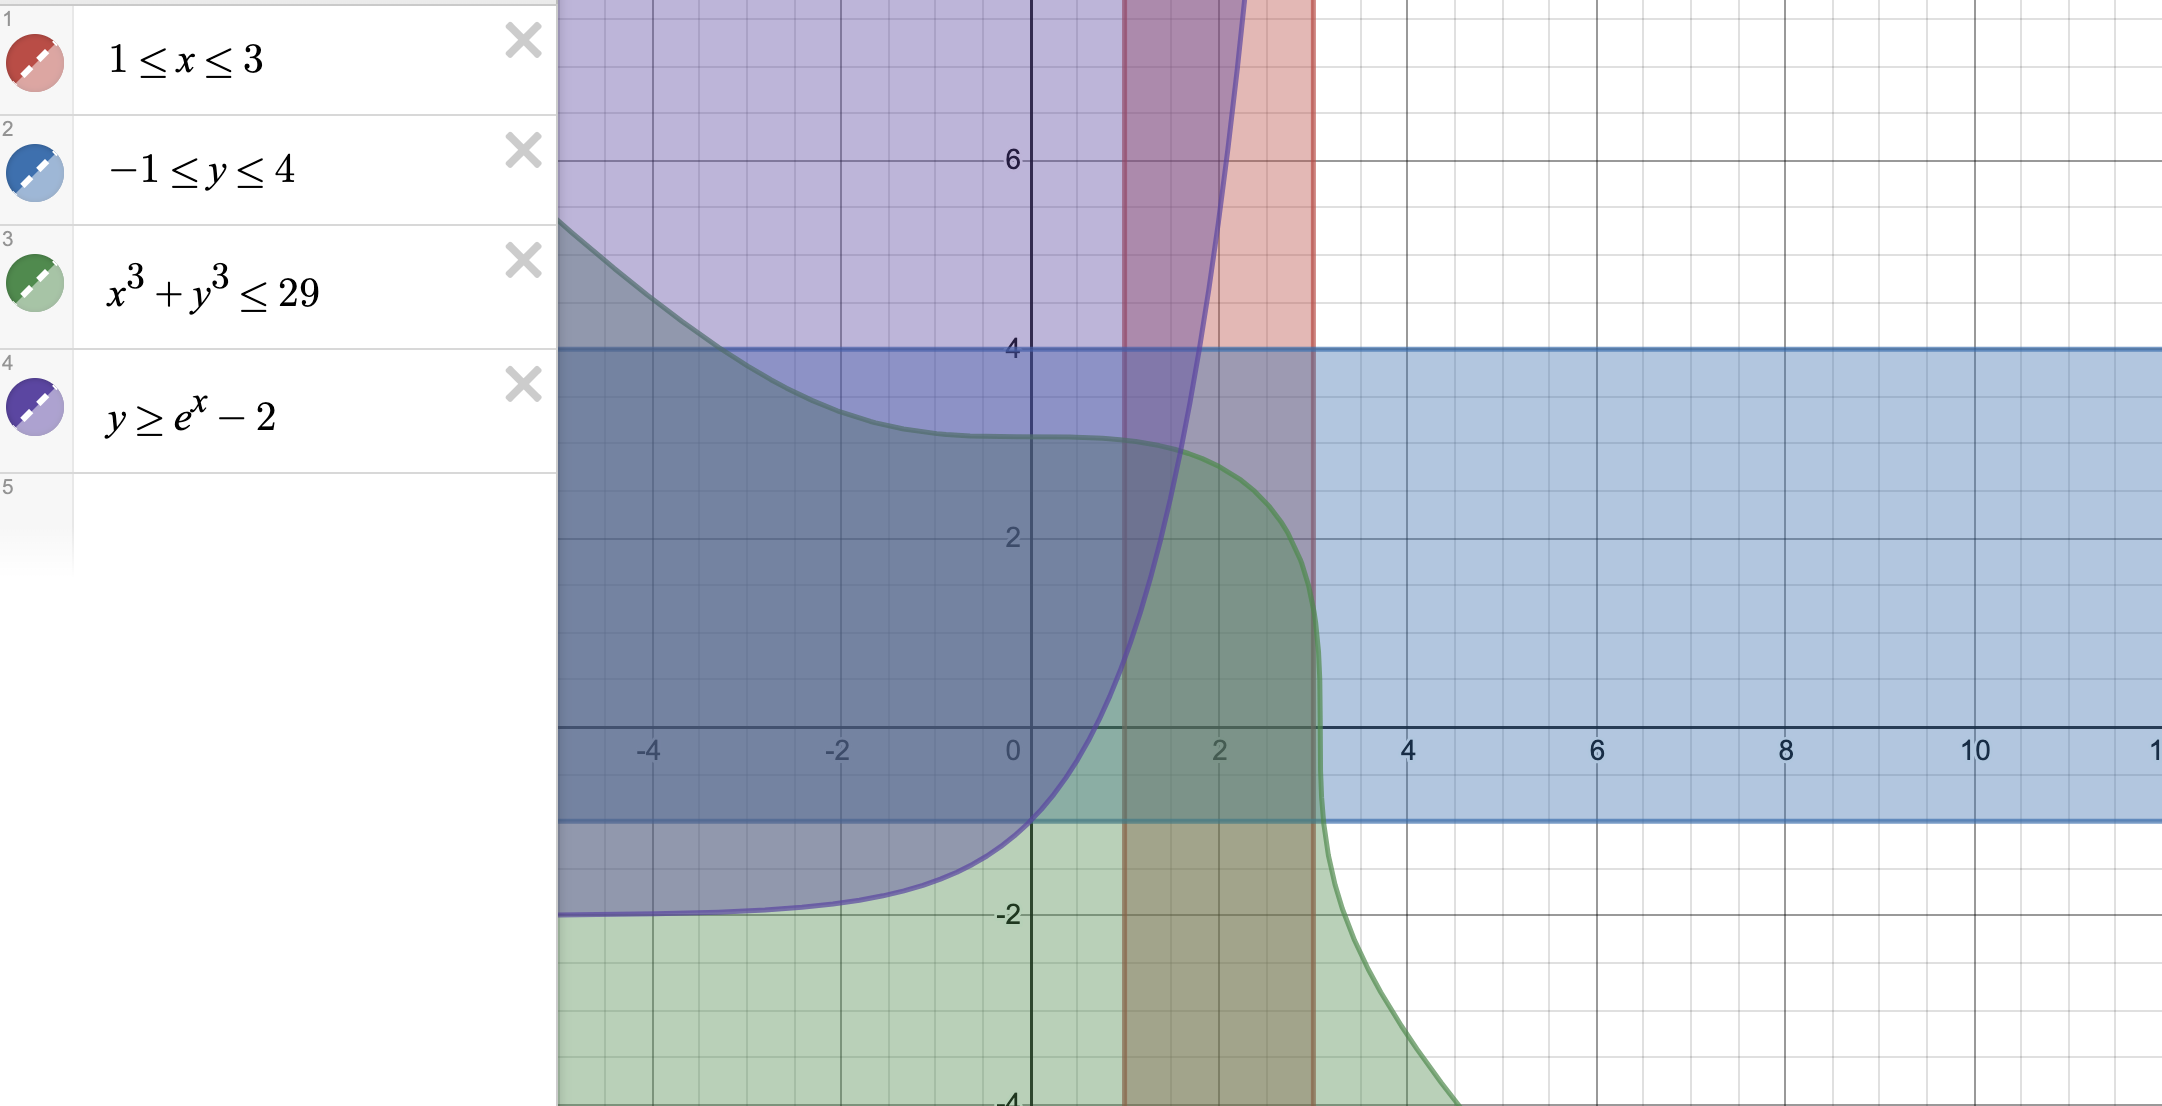
\includegraphics[width=\textwidth,height=\textheight,keepaspectratio]{desmos.png}
\section{Observations}
I can observe that the Monte Carlo method is pretty accurate if we compare the mathematical solution with the results obtained through the Intel MKL library. I can also observe that (at least in this experiment) reasonable precision is attained with only a moderate number of random numbers (1000) that with 1000 iterations leads to an average area of $7.692400000000001e-01$.

\end{document}